\section{Theory}
\label{sec:theory}
This section describes the theory behind the two main parts of the protocol that the IRMA Assurer protocol aims to connect. We start by providing insight into the IRMA eco system, followed by a quick overview of the ePassport security measures. Afterwards we sketch a typical run of the IRMA card application process.

\subsection{IRMA}
Here we explain the background of the IRMA proofs. IRMA stands for I Reveal My Attributes, which is a reference to attribute-based credentials (ABC) as described by~\cite{zeroknowledgeprotocols,abcfortrust,alpar2013credential}. ABCs (sometimes also referred to as anonymous credentials) are a way for people to share a part of their digital identity without disclosing any other information irrelevant to the goal of authentication. A digital identity is generally considered to be a set of characteristics describing particular properties about an individual. A distinction is made between identifying and non-identifying ABCs. Identifying ABCs are typically date of birth, name and social security number, whereas non-identifying ABCs may include hair color or favorite dish. Furthermore the set of ABCs is context-dependent and dynamic~\cite{abcofabc}. For the IRMA protocol only the identifying ABCs are relevant and use of the term ABC in the remainder of this document will refer only to this type.

In addition to the property it describes, any ABC is required to contain two additional basic attributes. First, an expiry date has to be determined at issuance, and it is included as an attribute applying to the whole credential. When the credential is verified, the expiry date can be revealed to confirm validity. Second, each user has a master secret key, stored in the smart card's secure storage, which is also incorporated -- technically, like an attribute -- in all credentials~\cite{alpar2013credential}.

Before it is possible to make use of ABCs for identification these first have to be provided by a third party, called an issuer. These issuers are parties who are allowed to give out ABCs. Any issuer cannot simply give out any ABC however. For example a bank may issue an ABC called `customer ID' for people who are customers with that particular bank, but may not issue credentials such as `date of birth' for the same people, or any other people for that matter. There are certain roles that issuers may assume and those they may not. Issuers determine the particular attributes they give out, but are verified by a scheme manager. Such a scheme manager effectively facilitates purpose limitation and data minimisation.

To summarize, the ecosystem distinguishes four roles:
\begin{enumerate}
  \item \textbf{Users} are people who own a smart card that holds valid attributes; validity means that the attributes on the card are valid for the card holder (and are not expired).
  \item \textbf{Issuers} are the authorities that sign credentials with attributes and provide them to users. For  instance, citizen registration authorities are the obvious issuers of `over 18' attributes (and of many other attributes as well) and banks are authoritative issuers of bank account number attributes.
  \item \textbf{Verifiers} (also called \textbf{relying parties}) are the parties that verify a subset of the available attributes on a card in order to authorise a transaction. An example verifier is a website that wants to verify the attribute ‘over 18’ before it allows me to view a certain video online.
  \item The \textbf{scheme manager} is an independent, non-profit organisation that sets the rules for the different parties (users, issuers and verifiers) and is responsible for the software and smart card management.
\end{enumerate}

Effectively an ABC can be seen as a secure container in which a characteristic from one's digital identity is stored. The attribute values are verified by issuer to ensure they match the individual's characteristics. Once a characteristic is verified the issuer will cryptographically sign the corresponding attribute and store it in the container. A municipality may for instance issue ABCs that state your place of birth and date of birth, which can then be checked by relying parties that require access to this information.

The benefit of using ABCs in favor of regular identification via say passports is the fact that it allows for selective disclosure of attributes. This enhances the privacy of your (digital) identity by not revealing anything that is not strictly necessary. Consider the following example. An individual wishes to rent a movie that contains violence. These movies typically require a minimum age. In the Netherlands such movies require you to be at least 18 years of age. When you wish to rent such a movie, the cashier asks you to prove you are at least 18 years old. ABCs allow you to digitally tell the cashier that you are `at least 18 years old' and are allowed to rent the movie. Note that the cashier never learns your actual age.

As stated above the IRMA project makes use of these ABCs, but mainly focusses on efficiency and practical issues when employing them~\cite{abcofabc}. All applicants receive a smart card that only features a photo of the card holder on the front. No further personally identifiable information is visible on the card.

An IRMA (smart) card is the physical container of attributes. As you can see below, the card shows only a picture of its holder but no other personal data. This is important for privacy and security reasons.

\begin{figure}[!ht]
  \centering
  \subfloat[Front\label{subfig:irma-front}]{%
    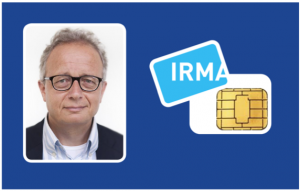
\includegraphics[width=0.45\textwidth]{images/IRMA_card_front.png}
  }
  \subfloat[Back\label{subfig:irma-back}]{%
    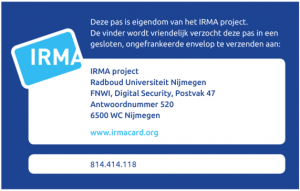
\includegraphics[width=0.45\textwidth]{images/IRMA_card_back.png}}
  \caption{IRMA card}
  \label{fig:dummy}
\end{figure}

\begin{enumerate}
	\item Your photo enables others to verify that the card belongs to you.
  \item In many situations it is not necessary to reveal your name or date of birth. That’s why they are not printed on the card. However, the card may contain these values digitally, stored as attributes.
  \item On the back of the card there is a card number. This number is only used for card administration. For instance, when a new card is handed over to a user, it is easy to find it based on this number.
  \item The card number is in not visible, but stored digitally inside the card.
\end{enumerate}

\subsection{Passport}
\label{subsec:passports}
\begin{wrapfigure}{R}{0.20\textwidth}
  \centering
	
\includegraphics[width=0.15\textwidth]{images/biometrics_logo.pdf}
	\caption{Symbol to indicate a biometric passport}
	\label{fig:biometricslogo}
\end{wrapfigure}
The passport is a travel document issued by a country's government that certifies the identity and nationality of its holder for the purpose of international travel~\cite{passportdefinition}. A biometric passport is an upgraded version that contains biometric information that can be used to authenticate the identity of travelers. This information is stored on an embedded chip that can be read using contactless smart card technology. Passports that feature such a chip generally feature the symbol shown in figure~\ref{fig:biometricslogo} on the cover. The data stored on the passport chip needs to be protected from modification, cloning, eavesdropping, etc. For this purpose several protection mechanisms have been implemented. Each of these mechanisms exists alongside each other and protects against different types of attacks. This section provides a brief overview of the various security protocols supported by passports, i.e. PA, BAC, SM and AA as specified by ICAO in~\cite{icao} as well as EAC as specified in~\cite{bsi}. 

\subsubsection{Passive Authentication}
\label{subsubsec:pa}
Passive Authentication (PA) is not actually a protocol. It simply indicates that the chip makes use of digital signatures of its data. PA involves the terminal reading the data and verifying both its hash and signature. PA is the only `protocol' that is ICAO mandatory; all other protocols are optional~\cite{mostowski2010electronic}.

\subsubsection{Basic Access Control}
Consider the case where a passport does not feature an RF chip. In this scenario privacy of the passport data is achieved by being able to keep the passport closed so nobody can read its data. With the addition of the RF chip this would no longer hold. Anyone with an RF reader (often called a terminal) is able to read the data on the chip if it is in close proximity. The solution to this problem is to protect the data with a key that the reader needs to know before being allowed to read the data. This is how the Basic Access Control (BAC) protocol works. BAC is essentially not required to be used by ePassports, but is strongly recommended. In the European Union however the use of BAC is mandatory~\cite{icao}. The key used for BAC is derived from three properties of the passport.
\begin{enumerate}
	\item The document number (usually 9 digits)
  \item The date of birth (formatted YYMMDD in Dutch passports)
  \item The document expiry date (formatted YYMMDD in Dutch passports)
\end{enumerate}
These three properties are part of the Machine Readable Zone (MRZ) that is printed in monospace at the bottom of the passport (see figure~\ref{fig:dutchpassport}). Also part of the MRZ is the Burger Service Nummer (BSN), which uniquely identifies a Dutch citizen, but this number is not used for the key derivation for BAC. Combining the aforementioned properties eventually results in the key with which the reader may access the chip's data. Keep in mind the MRZ is not visible while the passport is closed and cannot be obtained without opening the passport. Strictly speaking the MRZ could be obtained from the citizen database, but additional security checks are in place before it can be accessed. The only method of transferring the MRZ to the reader is for the reader to either utilize optical character recognition (OCR) software or for the passport holder to manually enter the information into the reader. In either case the MRZ is transmitted via an out of band channel. After the key is used for authenticating the reader to the passport, all further communication is performed via an encrypted channel using a session key~\cite{icao}.

In some countries, e.g. the US, the chip is shielded by a very thin metal mesh that is integrated into the cover of the passport~\cite{encuspassports}. This prevents readers from accessing the chip without having the passport holder open his or her passport first.

\subsubsection{Supplemental Access Control}
Supplemental Access Control (SAC) was introduced by ICAO in 2009 for addressing BAC weaknesses. It was introduced as a supplement to BAC (for keeping compatibility), but will replace it in the future. In principle it is a set of security features, which specifies the Password Authenticated Connection Establishment (PACE) protocol~\cite{icao}. PACE is preferred over BAC if it is implemented by a passport. It also derives the session key from the MRZ, but also allows key derivation from the Card Access Number (CAN) that is also present on the front of passports. The protocol uses a weak password (possibly of low entropy), verifies the password, and generates cryptographically strong session keys. It is mandatory from December 2014 onwards~\cite{gemalto}.

The PACE protocol comprises four steps:
\begin{enumerate}
	\item The chip randomly chooses a random number, encrypts it with a password-derived key and sends the encrypted random number to the terminal, where it is recovered.
  \item Both the chip and the terminal use a mapping function to map the random number to parameters for asymmetric cryptography. 
  \item The chip and the terminal perform a Diffie-Hellman protocol based on the parameters generated during step 2. 
  \item The chip and terminal derive session keys, which are confirmed by exchanging and checking the authentication tokens.
\end{enumerate}

\begin{figure}[htb]
	\centering
		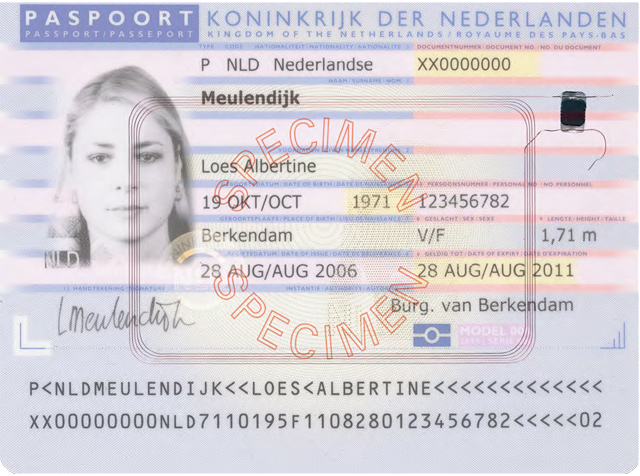
\includegraphics[width=0.50\textwidth]{images/dutchpassport.png}
	\caption{Dutch passport including a Machine Readable Zone at the bottom}
	\label{fig:dutchpassport}
\end{figure}

\subsubsection{Secure Messaging}
The Secure Messaging (SM) protocol is used to protect the integrity and confidentiality of the communication between terminal and chip. Essentially the protocol sets up a secure channel, the key for which is agreed upon during the BAC or PACE protocol. When also performing EAC, the CA part will refresh the key (see below).

\subsubsection{Extended Access Control}
Starting in 2006 many countries added their citizens' finger prints and iris scans to the chip, by definition turning it into a biometric passport. The biometric data is a lot more sensitive than the data protected by BAC, meaning it needs to be protected by stronger cryptography. For this the Extended Access Control (EAC) protocol was developed and added to the second generation of ePassports in 2009~\cite{gemalto}. Any reader that has successfully performed BAC may subsequently perform EAC in order to obtain access to the finger print and iris of the passport holder. EAC is implemented in all new generation EU passports, but nowhere else.

EAC consists of two protocols, Chip Authentication (CA) and Terminal Authentication (TA), both relying on a public key infrastructure (PKI) in which certificates are issued to the passport as well as other governments for verification purposes. The CA protocol is used for the terminal to authenticate the chip. It is based on a secret key agreement and a successful run of the protocol provides both parties with a new key for SM. The TA protocol is used for authenticating the terminal to the chip and possibly increase access rights. It actively verifies certificates. After both protocols have finished, mutual authentication is achieved and a new secure channel is created.

\subsubsection{Active Authentication}
Active Authentication (AA) is a challenge-response protocol that proves the authenticity of the chip, verifying the chip has not been cloned. The chip contains a private key, of which the chip proves knowledge during AA, and a certificate for this key as signed by the passport issuing country. This protocol is redundant when the passport also supports EAC, since the CA protocol also (implicitly) proves knowledge of this private key~\cite{secprivepassport}. This means that AA is only useful in cases where passports do not support EAC, but still wish to verify knowledge of the private key.

An example scenario of AA would be a passport that has a private key securely embedded in its chip. The public counterpart of this key is then signed by the passport's producer, Morpho\footnote{\url{http://www.morpho.com/}} in the Netherlands. Morpho's public key is subsequently signed by the Dutch government, creating a certificate chain. Sending a challenge to the chip, encrypted with its public key would allow the chip to solve the challenge by decrypting it using its private key and thus proving its identity to the terminal.

\subsection{Usage scenario}
\label{subsec:bcoe}
This section describes the basic course of events when a citizen requests a personal IRMA card and would like it to be initialized with his or her passport information. Here we only mention assumptions of operational nature. Goals and assumptions of cryptographic nature are discussed in section~\ref{sec:assumptions}. 

First of all we assume the citizen in question is an inhabitant of the Netherlands and is in possession of an electronic passport. The citizen will fill out an online application form and enclose a photo in order to request a new IRMA card. Once the application is received by the IRMA card manufacturer a new IRMA card will be created. This card is blank, i.e. there are no attributes on the card. The application for this card, as well as the blank card itself, will subsequently be forwarded to one of several dozens of assurers. 

These assurers may be situated in a government building, for example in a town hall, or they could be notaries, or they might be something else entirely as long as they are public figures who either directly or indirectly work for the government. Assurers are in possession of a tablet device that contains a Near-Field Communication (NFC) chip that allows for contactless communication with the IRMA card. This tablet will be kept under lock and key in a safe and is protected with a PIN in order to prevent unauthorized use. At each location only one person (a few at most) will be in posession of this key and PIN. The citizen will go to one of these assurers and present his or her passport to the tablet if the assurer confirms that the uploaded photo, which is printed on the front of the IRMA card, matches the citizen. 

The data on the passport is verified by the tablet and if confirmed to be valid will be sent to a (the only) central server. The server repeats these checks and also performs several additional checks to definitively verify the passport. Such additional checks may include absence of this particular passport in the database of stolen and lost passports. The server will then proceed to convert the passport's data into attribute data. These attributes are cryptographically signed by the server, who is the only party in posession of the private part of the only attribute signing keypair, i.e. the issuer keypair. Once the passport data is converted into attribute data the server sends the attributes back to the assurer's tablet. The server keeps a log of the BSN stored in the passport data plus the time of the request, but deletes all other traces of the data (both passport and attribute) once it has been received by the assurer's tablet. 

The attribute data is received by the tablet and the assurer asks the citizen to present his or her IRMA card. The attribute data is subsequently written to the IRMA card by the tablet. Upon successful transfer of the attribute data, all traces of the entire transaction are deleted from the tablet. The citizen has now successfully added the data from his or her passport to the newly created IRMA card.
